% !TeX program = XeLaTeX
\documentclass[11pt]{article}\usepackage[]{graphicx}\usepackage[]{color}
% maxwidth is the original width if it is less than linewidth
% otherwise use linewidth (to make sure the graphics do not exceed the margin)
\makeatletter
\def\maxwidth{ %
  \ifdim\Gin@nat@width>\linewidth
    \linewidth
  \else
    \Gin@nat@width
  \fi
}
\makeatother

\definecolor{fgcolor}{rgb}{0.196, 0.196, 0.196}
\makeatletter
\@ifundefined{AddToHook}{}{\AddToHook{package/xcolor/after}{\definecolor{fgcolor}{rgb}{0.196, 0.196, 0.196}}}
\makeatother
\newcommand{\hlnum}[1]{\textcolor[rgb]{0.063,0.58,0.627}{#1}}%
\newcommand{\hlstr}[1]{\textcolor[rgb]{0.063,0.58,0.627}{#1}}%
\newcommand{\hlcom}[1]{\textcolor[rgb]{0.588,0.588,0.588}{#1}}%
\newcommand{\hlopt}[1]{\textcolor[rgb]{0.196,0.196,0.196}{#1}}%
\newcommand{\hlstd}[1]{\textcolor[rgb]{0.196,0.196,0.196}{#1}}%
\newcommand{\hlkwa}[1]{\textcolor[rgb]{0.231,0.416,0.784}{#1}}%
\newcommand{\hlkwb}[1]{\textcolor[rgb]{0.627,0,0.314}{#1}}%
\newcommand{\hlkwc}[1]{\textcolor[rgb]{0,0.631,0.314}{#1}}%
\newcommand{\hlkwd}[1]{\textcolor[rgb]{0.78,0.227,0.412}{#1}}%
\let\hlipl\hlkwb

\usepackage{framed}
\makeatletter
\newenvironment{kframe}{%
 \def\at@end@of@kframe{}%
 \ifinner\ifhmode%
  \def\at@end@of@kframe{\end{minipage}}%
  \begin{minipage}{\columnwidth}%
 \fi\fi%
 \def\FrameCommand##1{\hskip\@totalleftmargin \hskip-\fboxsep
 \colorbox{shadecolor}{##1}\hskip-\fboxsep
     % There is no \\@totalrightmargin, so:
     \hskip-\linewidth \hskip-\@totalleftmargin \hskip\columnwidth}%
 \MakeFramed {\advance\hsize-\width
   \@totalleftmargin\z@ \linewidth\hsize
   \@setminipage}}%
 {\par\unskip\endMakeFramed%
 \at@end@of@kframe}
\makeatother

\definecolor{shadecolor}{rgb}{.97, .97, .97}
\definecolor{messagecolor}{rgb}{0, 0, 0}
\definecolor{warningcolor}{rgb}{1, 0, 1}
\definecolor{errorcolor}{rgb}{1, 0, 0}
\makeatletter
\@ifundefined{AddToHook}{}{\AddToHook{package/xcolor/after}{
\definecolor{shadecolor}{rgb}{.97, .97, .97}
\definecolor{messagecolor}{rgb}{0, 0, 0}
\definecolor{warningcolor}{rgb}{1, 0, 1}
\definecolor{errorcolor}{rgb}{1, 0, 0}
}}
\makeatother
\newenvironment{knitrout}{}{} % an empty environment to be redefined in TeX

\usepackage{amsmath}
\usepackage{alltt}
\usepackage{fontspec,xunicode}
\usepackage[no-sscript]{xltxtra}
%\setmainfont[Mapping=tex-text]{Garamond Normal}
\setmonofont[Scale=0.8]{Consolas}
\setmathrm{Optima}
\setboldmathrm[BoldFont=Optima ExtraBlack]{Optima Bold}
\usepackage{polyglossia}
\setdefaultlanguage{french}
\usepackage{amsmath,amssymb,colortbl,calc,listings,graphicx,color,makeidx,nonfloat,url,multicol}
%\usepackage{numprint}
\usepackage{siunitx}
\sisetup{
locale = FR,
round-mode = places,
round-precision = 3
}
\setcounter{tocdepth}{2}
\definecolor{RedOrange}{cmyk}{0.8, 0.5, 0, 0.3}
\definecolor{graym}{rgb}{0.96, 0.96, 0.96}
\usepackage{caption}
\captionsetup{labelfont={color=RedOrange,bf},textfont={color=RedOrange,it}}
\usepackage[colorlinks=true,plainpages=true,linktocpage,hyperindex=true,citecolor=RedOrange,linkcolor=RedOrange,urlcolor=RedOrange]{hyperref}
\usepackage{titlesec, blindtext, color}
\definecolor{gray75}{gray}{0.75}
\newcommand{\hsp}{\hspace{20pt}}
\newcommand{\type}[1]{\textcolor{RedOrange}{\texttt{#1}}}
\titleformat{\chapter}[hang]{\Huge\bfseries}{\thechapter\hsp\textcolor{gray75}{|}\hsp}{0pt}{\Huge\bfseries}
\textwidth 16cm
\textheight 23cm
\topmargin -1.9cm
\oddsidemargin .4cm
\evensidemargin .2cm
\marginparsep .5cm
\footskip 1.5cm
\headsep 1.5cm
\marginparwidth 2cm
\IfFileExists{upquote.sty}{\usepackage{upquote}}{}
\begin{document}

%#F7F7F7




\begin{center}
\vspace{-1.5cm}
%\scalebox{.18}{\includegraphics{img/ifsttar.pdf}}

\vspace{2cm}
{\Large \textbf{CODE R POUR SONOREZÉ}}


\vspace{4cm}
4 janvier 2022

\textcolor{RedOrange}{\rule{2.75cm}{.3pt}}

\vspace{.3cm}
{\large \textbf{Tristan Lorino}}
\end{center}
\thispagestyle{empty}

\vspace*{3cm}
\tableofcontents

\newpage
\section{Préalable}

On commence par créer un projet RStudio qui sera contenu dans un dossier (déjà existant ou à créer).
Dans ce dossier, on créé un dossier nommé \type{R} dans lequel on va stocker trois scripts R, qui seront à \textbf{exécuter dans cet ordre l'un après l'autre} : \type{import\_database.R}, \type{Statistiques-v2.R} et \type{Graphiques.R}.

Le fichier \type{import\_database.R} se charge en premier lieu de télécharger et installer un package nommé \type{pacman}, qui va se charger d'importer si besoin, et de charger tous les autres packages nécessaires à l'exécution des scripts R.

\begin{knitrout}\footnotesize
\definecolor{shadecolor}{rgb}{0.91, 0.91, 0.91}\color{fgcolor}\begin{kframe}
\begin{alltt}
\hlkwd{install.packages}\hlstd{(}\hlstr{"pacman"}\hlstd{)}
\hlkwd{library}\hlstd{(pacman)}
\hlstd{pacman}\hlopt{::}\hlkwd{p_load}\hlstd{(thematic,lubridate,dplyr,tidyr,stringr,ggplot2,forcats,rgdal,sp,sf,}
               \hlstd{rgeos,tidyr,devtools,leaflet,leaflet.extras,jsonlite,RColorBrewer,}
               \hlstd{viridis,forcats,mapview,scales)}
\end{alltt}
\end{kframe}
\end{knitrout}

\section{Importation des données}



Le fichier \type{import\_database.R} permet d'importer les données NoiseCapture relatives au projet Sonorezé.

Il nécessite l'emploi de quatre package : \type{\{here\}} pour utiliser des chemins relatifs dans le projet R, \type{\{lubridate\}} pour une utilisation poussée des dates, \type{\{dplyr\}} pour une gestion avancée des commandes et \type{\{stringr\}} pour une gestion poussée des chaînes de caractères.

Il faut au préalable créer un dossier (ou répertoire) \type{metabase} dans le dossier du projet RStudio. L'exécution du script R va créer un dossier \type{data} dans \type{metabase}, puis un dossier \type{unzip} dans \type{data}. Tous les fichiers zippés des traces vont être stockés dans \type{data}, puis vont être dézippés dans \type{unzip} : chaque extraction d'archive donne lieu à la création d'un dossier. Finalement on obtient, pour chaque trace, un dossier contenant deux fichiers : \type{meta.properties} et \type{track.geojson}.

On extrait ensuite :
\begin{itemize}
\item du fichier \type{meta.properties} : les champs \type{uuid} (pour lequel on ne conserve que les quatre premiers caractères), \type{Gain\_calibration} et \type{method\_calibration} ;

\begin{knitrout}\footnotesize
\definecolor{shadecolor}{rgb}{0.91, 0.91, 0.91}\color{fgcolor}\begin{kframe}
\begin{alltt}
\hlstd{uuid} \hlkwb{<-} \hlstd{meta} \hlopt
        \hlkwd{filter}\hlstd{(}\hlkwd{startsWith}\hlstd{(V1,} \hlstr{'uuid='}\hlstd{))} \hlopt
        \hlkwd{str_sub}\hlstd{(.,} \hlnum{6}\hlstd{,} \hlnum{9}\hlstd{)}

      \hlstd{gain_cal}\hlkwb{<-} \hlstd{meta} \hlopt
        \hlkwd{filter}\hlstd{(}\hlkwd{startsWith}\hlstd{(V1,} \hlstr{'gain_calibration='}\hlstd{))} \hlopt
        \hlkwd{str_remove}\hlstd{(.,} \hlstr{"gain_calibration="}\hlstd{)}

      \hlstd{method_cal}\hlkwb{<-} \hlstd{meta} \hlopt
        \hlkwd{filter}\hlstd{(}\hlkwd{startsWith}\hlstd{(V1,} \hlstr{'method_calibration='}\hlstd{))} \hlopt
        \hlkwd{str_remove}\hlstd{(.,} \hlstr{"method_calibration="}\hlstd{)}
\end{alltt}
\end{kframe}
\end{knitrout}

\item du fichier \type{track.geojson} : les champs \type{leq\_utc} (exprimé au format epoch, il est converti en date UTC), ceux des mesures de bruit pour les différentes fréquences, le Leq moyen, les coordonnées GPS et la précision (\textit{accuracy}).
\end{itemize}

\begin{knitrout}\footnotesize
\definecolor{shadecolor}{rgb}{0.91, 0.91, 0.91}\color{fgcolor}\begin{kframe}
\begin{alltt}
\hlstd{data} \hlkwb{<-} \hlstd{data[}\hlkwd{c}\hlstd{(}\hlstr{"leq_100"}\hlstd{,} \hlstr{"leq_125"}\hlstd{, ...,}\hlstr{"leq_12500"}\hlstd{,}\hlstr{"leq_16000"}\hlstd{,}\hlstr{"leq_mean"}\hlstd{,}\hlstr{"x"}\hlstd{,}\hlstr{"y"}\hlstd{,}\hlstr{"leq_utc"}\hlstd{,}\hlstr{"accuracy"}\hlstd{)]}
\end{alltt}
\end{kframe}
\end{knitrout}



0n va ensuite repositionner en première place les colonnes \type{Id, Date, x} et \type{y}, puis assembler ces différentes informations pour n'avoir plus qu'un seul tableau de données nommés \type{noisecapture\_data}, que l'on va stocker dans le répertoire courant sous le nom \type{noisecapture\_data.Rda}.

\begin{knitrout}\footnotesize
\definecolor{shadecolor}{rgb}{0.91, 0.91, 0.91}\color{fgcolor}\begin{kframe}
\begin{alltt}
\hlstd{temp} \hlkwb{<-} \hlstd{data} \hlopt
        \hlkwd{mutate}\hlstd{(}\hlkwc{Date} \hlstd{= lubridate}\hlopt{::}\hlkwd{as_datetime}\hlstd{(.}\hlopt{$}\hlstd{leq_utc}\hlopt{/}\hlnum{1000}\hlstd{,} \hlkwc{tz}\hlstd{=}\hlstr{"UTC"}\hlstd{))} \hlopt
        \hlkwd{select}\hlstd{(}\hlopt{!}\hlstd{leq_utc)} \hlopt
        \hlkwd{mutate}\hlstd{(}\hlkwc{Id}\hlstd{=uuid)} \hlopt
        \hlkwd{mutate}\hlstd{(}\hlkwc{gain_calibration}\hlstd{=gain_cal)} \hlopt
        \hlkwd{mutate}\hlstd{(}\hlkwc{method_calibration}\hlstd{=method_cal)} \hlopt
        \hlkwd{relocate}\hlstd{(Id,Date,x,y)}

      \hlstd{noisecapture_data} \hlkwb{<-} \hlkwd{bind_rows}\hlstd{(temp, noisecapture_data)}
      \hlstd{noisecapture_data}
      \hlkwd{save}\hlstd{(noisecapture_data,} \hlkwc{file} \hlstd{=}\hlstr{"noisecapture_data.Rda"}\hlstd{)}
\end{alltt}
\end{kframe}
\end{knitrout}


%%%%%%%%%%%%%%%%%%%%%%%%%%
\newpage
\section{Statistiques}

\subsection{Introduction}

Outre les packages précédemment cités, on charge en plus le package \type{\{forcats\}}, qui permet de recoder facilement les modalités d'un facteur.

En premier lieu, on regarde le nombre de mesures (enregistrements au pas d'une seconde) réalisées. Il y en a :
\begin{knitrout}\footnotesize
\definecolor{shadecolor}{rgb}{0.91, 0.91, 0.91}\color{fgcolor}\begin{kframe}
\begin{alltt}
\hlkwd{load}\hlstd{(}\hlkwd{here}\hlstd{(}\hlstr{"noisecapture_data.Rda"}\hlstd{))}
\hlstd{data_nc} \hlkwb{<-}\hlkwd{as.data.frame}\hlstd{(noisecapture_data)}
\hlkwd{dim}\hlstd{(data_nc)[}\hlnum{1}\hlstd{]}
\end{alltt}
\begin{verbatim}
## [1] 0
\end{verbatim}
\end{kframe}
\end{knitrout}

Ensuite on détecte les valeurs manquantes pour les coordonnées GPS, ainsi que les éventuelles dates aberrantes. Il y en a :
\begin{knitrout}\footnotesize
\definecolor{shadecolor}{rgb}{0.91, 0.91, 0.91}\color{fgcolor}\begin{kframe}
\begin{alltt}
\hlstd{databer} \hlkwb{<-} \hlstd{data_nc[data_nc}\hlopt{$}\hlstd{Date} \hlopt{<} \hlstr{"2021-11-01 00:00:01"} \hlopt{|} \hlstd{data_nc}\hlopt{$}\hlstd{x} \hlopt{==} \hlstr{"NA"} \hlopt{|} \hlstd{data_nc}\hlopt{$}\hlstd{y} \hlopt{==}\hlstr{"NA"}\hlstd{,]}
\hlkwd{dim}\hlstd{(databer)[}\hlnum{1}\hlstd{]}
\end{alltt}
\begin{verbatim}
## [1] 0
\end{verbatim}
\end{kframe}
\end{knitrout}

On calcule ensuite le nombre de mesures avec une précision supérieure à 20. Il y en a :
\begin{knitrout}\footnotesize
\definecolor{shadecolor}{rgb}{0.91, 0.91, 0.91}\color{fgcolor}\begin{kframe}
\begin{alltt}
\hlstd{data_accuracy} \hlkwb{<-} \hlstd{data_nc[data_nc}\hlopt{$}\hlstd{accuracy} \hlopt{>=} \hlnum{20}\hlstd{,]}
\hlkwd{dim}\hlstd{(data_accuracy)}
\end{alltt}
\begin{verbatim}
## [1] 0 0
\end{verbatim}
\end{kframe}
\end{knitrout}

Si l'on retire les mesures avec données manquantes ou précision insuffisante, on retient :
\begin{knitrout}\footnotesize
\definecolor{shadecolor}{rgb}{0.91, 0.91, 0.91}\color{fgcolor}\begin{kframe}
\begin{alltt}
\hlstd{data_nc} \hlkwb{<-} \hlstd{data_nc} \hlopt
  \hlkwd{filter}\hlstd{(x} \hlopt{!=} \hlstr{"NA"}\hlstd{)} \hlopt
  \hlkwd{filter}\hlstd{(accuracy}\hlopt{<}\hlnum{20}\hlstd{)}
\end{alltt}


{\ttfamily\noindent\bfseries\color{errorcolor}{\#\# Error: Problem with `filter()` input `..1`.\\\#\# i Input `..1` is `x != "{}NA"{}`.\\\#\# x objet 'x' introuvable}}\begin{alltt}
\hlkwd{dim}\hlstd{(data_nc)[}\hlnum{1}\hlstd{]}
\end{alltt}
\begin{verbatim}
## [1] 0
\end{verbatim}
\end{kframe}
\end{knitrout}
soit $97{,}3$~\% des mesures.

\subsection{Statistiques relatives aux mesures}

On va créer différents tableaux de données :
\begin{itemize}
\item un nommé \type{AnaMes} pour le nombre de mesures par participants, avec pourcentage sur l'ensemble :
\begin{knitrout}\footnotesize
\definecolor{shadecolor}{rgb}{0.91, 0.91, 0.91}\color{fgcolor}\begin{kframe}
\begin{alltt}
\hlstd{AnaMes} \hlkwb{<-} \hlstd{data_nc} \hlopt
  \hlkwd{group_by}\hlstd{(Id)} \hlopt
  \hlkwd{summarise}\hlstd{(}\hlkwc{n} \hlstd{=} \hlkwd{n}\hlstd{())} \hlopt
  \hlkwd{mutate}\hlstd{(}\hlkwc{Pourcentage}\hlstd{=n}\hlopt{/}\hlkwd{sum}\hlstd{(n)}\hlopt{*}\hlnum{100}\hlstd{)} \hlopt
  \hlkwd{arrange}\hlstd{(}\hlkwd{desc}\hlstd{(n))}
\end{alltt}
\end{kframe}
\end{knitrout}

\item  un nommé \type{data\_mes}, qui correspond à \type{data\_nc}, auquel on ajoute deux champs, \type{DateJour} et \type{DateHeure} :
\begin{knitrout}\footnotesize
\definecolor{shadecolor}{rgb}{0.91, 0.91, 0.91}\color{fgcolor}\begin{kframe}
\begin{alltt}
\hlstd{data_mes} \hlkwb{<-} \hlstd{data_nc} \hlopt
  \hlkwd{mutate}\hlstd{(}\hlkwc{DateJour}\hlstd{=}\hlkwd{as.Date}\hlstd{(Date))} \hlopt
  \hlkwd{mutate}\hlstd{(}\hlkwc{DateHeure}\hlstd{=}\hlkwd{hour}\hlstd{(}\hlkwd{as.POSIXct}\hlstd{(Date)))}
\hlstd{data_mes}
\end{alltt}
\end{kframe}
\end{knitrout}

\item l'évolution du nombre de mesures par jour :
\begin{knitrout}\footnotesize
\definecolor{shadecolor}{rgb}{0.91, 0.91, 0.91}\color{fgcolor}\begin{kframe}
\begin{alltt}
\hlstd{data_mes_jour} \hlkwb{<-} \hlkwd{as.data.frame}\hlstd{(data_mes)} \hlopt
  \hlkwd{group_by}\hlstd{(DateJour)} \hlopt
  \hlkwd{summarise}\hlstd{(}\hlkwc{NbMes} \hlstd{=} \hlkwd{n}\hlstd{())} \hlopt
  \hlkwd{mutate}\hlstd{(}\hlkwc{NbMesCum}\hlstd{=}\hlkwd{cumsum}\hlstd{(NbMes))}
\end{alltt}
\end{kframe}
\end{knitrout}

\item l'évolution du nombre de participants par jour :
\begin{knitrout}\footnotesize
\definecolor{shadecolor}{rgb}{0.91, 0.91, 0.91}\color{fgcolor}\begin{kframe}
\begin{alltt}
\hlstd{data_ind} \hlkwb{<-} \hlstd{data_mes} \hlopt
  \hlkwd{group_by}\hlstd{(DateJour)} \hlopt
  \hlkwd{summarise}\hlstd{(}\hlkwc{NbId} \hlstd{=} \hlkwd{n_distinct}\hlstd{(Id))}
\end{alltt}
\end{kframe}
\end{knitrout}
\end{itemize}


\subsection{Statistiques relatives aux traces}

À partir du tableau de données \type{data\_mes}, on créé un tableau de donnnées \type{data\_trace} avec :
\begin{itemize}
\item un identifiant des traces (plage de mesures consécutives) :
\begin{knitrout}\footnotesize
\definecolor{shadecolor}{rgb}{0.91, 0.91, 0.91}\color{fgcolor}\begin{kframe}
\begin{alltt}
\hlstd{data_trace} \hlkwb{<-} \hlkwd{as.data.frame}\hlstd{(data_mes)} \hlopt
  \hlkwd{arrange}\hlstd{(Id,Date)} \hlopt
  \hlkwd{mutate}\hlstd{(}\hlkwc{IdTrace}\hlstd{=}\hlkwd{cumsum}\hlstd{(}\hlkwd{c}\hlstd{(}\hlnum{TRUE}\hlstd{,} \hlkwd{as.integer}\hlstd{(}\hlkwd{diff}\hlstd{(}\hlkwd{as.POSIXct}\hlstd{(Date)),} \hlkwc{units} \hlstd{=} \hlstr{"secs"}\hlstd{)} \hlopt{>=} \hlnum{2L}\hlstd{)))}
\end{alltt}
\end{kframe}
\end{knitrout}

\item deux variables relatives au jour, \type{DateJour} le jour sous la forme de date entière et \type{DateJourSem} le jour sous forme de jour de la semaine :
\begin{knitrout}\footnotesize
\definecolor{shadecolor}{rgb}{0.91, 0.91, 0.91}\color{fgcolor}\begin{kframe}
\begin{alltt}
  \hlkwd{mutate}(DateJour=\hlkwd{as.Date}(Date)) %>%
  \hlkwd{mutate}(DateJourSem=\hlkwd{wday}(Date)) %>%
\end{alltt}
\end{kframe}
\end{knitrout}

\item et on calcule la durée de chaque trace en secondes et minutes :
\begin{knitrout}\footnotesize
\definecolor{shadecolor}{rgb}{0.91, 0.91, 0.91}\color{fgcolor}\begin{kframe}
\begin{alltt}
  \hlkwd{group_by}\hlstd{(IdTrace)} \hlopt
  \hlkwd{mutate}\hlstd{(}\hlkwc{DureeSec}\hlstd{=}\hlkwd{n}\hlstd{())} \hlopt
  \hlkwd{arrange}\hlstd{(Id,}\hlkwd{desc}\hlstd{(DureeSec))} \hlopt
  \hlkwd{mutate}\hlstd{(}\hlkwc{DureeMinutes}\hlstd{=DureeSec}\hlopt{/}\hlnum{60}\hlstd{)}
\end{alltt}
\end{kframe}
\end{knitrout}
\end{itemize}


Ensuite on calcule le nombre de traces par participants, avec pourcentage sur l'ensemble :
\begin{knitrout}\footnotesize
\definecolor{shadecolor}{rgb}{0.91, 0.91, 0.91}\color{fgcolor}\begin{kframe}
\begin{alltt}
\hlstd{data_trace} \hlopt
  \hlkwd{distinct}\hlstd{(IdTrace,} \hlkwc{.keep_all} \hlstd{=} \hlnum{TRUE}\hlstd{)} \hlopt
  \hlkwd{group_by}\hlstd{(Id)} \hlopt
  \hlkwd{summarise}\hlstd{(}\hlkwc{n} \hlstd{=} \hlkwd{n}\hlstd{())} \hlopt
  \hlkwd{mutate}\hlstd{(}\hlkwc{Pourcentage}\hlstd{=n}\hlopt{/}\hlkwd{sum}\hlstd{(n)}\hlopt{*}\hlnum{100}\hlstd{)} \hlopt
  \hlkwd{arrange}\hlstd{(}\hlkwd{desc}\hlstd{(n))}
\end{alltt}
\end{kframe}
\end{knitrout}

On créé ensuite une variable factorielle \type{Classe} pour des plages de durée :
\begin{knitrout}\footnotesize
\definecolor{shadecolor}{rgb}{0.91, 0.91, 0.91}\color{fgcolor}\begin{kframe}
\begin{alltt}
\hlstd{data_trace} \hlkwb{<-} \hlstd{data_trace} \hlopt
  \hlkwd{mutate}\hlstd{(}\hlkwc{Classe} \hlstd{=} \hlkwd{case_when}\hlstd{(DureeMinutes} \hlopt{<} \hlnum{5} \hlopt{~} \hlstr{"0-5"}\hlstd{,}
                            \hlstd{DureeMinutes} \hlopt{<} \hlnum{10} \hlopt{~} \hlstr{"5-10"}\hlstd{,}
                            \hlstd{DureeMinutes} \hlopt{<} \hlnum{15} \hlopt{~} \hlstr{"10-15"}\hlstd{,}
                            \hlstd{DureeMinutes} \hlopt{<} \hlnum{20} \hlopt{~} \hlstr{"15-20"}\hlstd{,}
                            \hlstd{DureeMinutes} \hlopt{<} \hlnum{25} \hlopt{~} \hlstr{"20-25"}\hlstd{,}
                            \hlstd{DureeMinutes} \hlopt{<} \hlnum{30} \hlopt{~} \hlstr{"25-30"}\hlstd{,}
                            \hlstd{DureeMinutes} \hlopt{<} \hlnum{35} \hlopt{~} \hlstr{"30-35"}\hlstd{,}
                            \hlstd{DureeMinutes} \hlopt{<} \hlnum{40} \hlopt{~} \hlstr{"35-40"}\hlstd{,}
                            \hlstd{DureeMinutes} \hlopt{<} \hlnum{45} \hlopt{~} \hlstr{"40-45"}\hlstd{,}
                            \hlstd{DureeMinutes} \hlopt{<} \hlnum{50} \hlopt{~} \hlstr{"45-50"}\hlstd{,}
                            \hlstd{DureeMinutes} \hlopt{<} \hlnum{55} \hlopt{~} \hlstr{"50-55"}\hlstd{,}
                            \hlstd{DureeMinutes} \hlopt{<} \hlnum{60} \hlopt{~} \hlstr{"55-60"}\hlstd{,}
                            \hlnum{TRUE} \hlopt{~} \hlstr{"> 60"}\hlstd{))} \hlopt
  \hlkwd{mutate}\hlstd{(}\hlkwc{Classe} \hlstd{=} \hlkwd{factor}\hlstd{(Classe))}
\end{alltt}
\end{kframe}
\end{knitrout}

Mais les modalités ne sont pas dans le bon ordre :
\begin{knitrout}\footnotesize
\definecolor{shadecolor}{rgb}{0.91, 0.91, 0.91}\color{fgcolor}\begin{kframe}
\begin{alltt}
\hlkwd{levels}(data_trace$Classe)
[1] \hlstr{"0-5"}   \hlstr{"> 60"}  \hlstr{"20-25"} \hlstr{"15-20"} \hlstr{"5-10"}
\end{alltt}
\end{kframe}
\end{knitrout}

Pour les réordonner, on fait appel au package \type{\{forcats\}} :
\begin{knitrout}\footnotesize
\definecolor{shadecolor}{rgb}{0.91, 0.91, 0.91}\color{fgcolor}\begin{kframe}
\begin{alltt}
data_trace <- data_trace %>%
  \hlkwd{mutate}(Classe = forcats::\hlkwd{fct_relevel}(Classe,\hlkwd{c}(\hlstr{"0-5"},\hlstr{"5-10"},\hlstr{"15-20"},\hlstr{"20-25"},\hlstr{"> 60"}))) %>%
  \hlkwd{arrange}(Classe)
\hlkwd{levels}(data_trace$Classe)

[1] \hlstr{"0-5"}   \hlstr{"5-10"}  \hlstr{"15-20"} \hlstr{"20-25"} \hlstr{"> 60"}
\end{alltt}
\end{kframe}
\end{knitrout}

On détermine ensuite l'évolution du nombre de traces par jour et en cumulé :
\begin{knitrout}\footnotesize
\definecolor{shadecolor}{rgb}{0.91, 0.91, 0.91}\color{fgcolor}\begin{kframe}
\begin{alltt}
\hlstd{data_trace_jour} \hlkwb{<-} \hlstd{data_trace} \hlopt
  \hlkwd{group_by}\hlstd{(DateJour)} \hlopt
  \hlkwd{distinct}\hlstd{(IdTrace,} \hlkwc{.keep_all} \hlstd{=} \hlnum{TRUE}\hlstd{)} \hlopt
  \hlkwd{summarise}\hlstd{(}\hlkwc{NbTraceParJour} \hlstd{=} \hlkwd{n}\hlstd{())} \hlopt
  \hlkwd{mutate}\hlstd{(}\hlkwc{NbTraceParJourCum}\hlstd{=}\hlkwd{cumsum}\hlstd{(NbTraceParJour))}
\end{alltt}
\end{kframe}
\end{knitrout}

Enfin on détermine l'évolution du nombre de traces par jour de la semaine :
\begin{knitrout}\footnotesize
\definecolor{shadecolor}{rgb}{0.91, 0.91, 0.91}\color{fgcolor}\begin{kframe}
\begin{alltt}
\hlstd{data_trace} \hlopt
  \hlkwd{group_by}\hlstd{(DateJourSem)} \hlopt
  \hlkwd{distinct}\hlstd{(IdTrace,} \hlkwc{.keep_all} \hlstd{=} \hlnum{TRUE}\hlstd{)} \hlopt
  \hlkwd{summarise}\hlstd{(}\hlkwc{NbTraceParJourSem} \hlstd{=} \hlkwd{n}\hlstd{())} \hlopt
  \hlkwd{mutate}\hlstd{(}\hlkwc{NbTracParJourSemCum}\hlstd{=}\hlkwd{cumsum}\hlstd{(NbTraceParJourSem))}
\end{alltt}
\end{kframe}
\end{knitrout}

%%%%%%%%%%%%%%%%%%%%%%%%%%
\newpage
\section{Graphiques}

\subsection{Généralités}

Pour avoir une virgule comme marque de décimale, on écrit :
\begin{knitrout}\footnotesize
\definecolor{shadecolor}{rgb}{0.91, 0.91, 0.91}\color{fgcolor}\begin{kframe}
\begin{alltt}
\hlkwd{options}\hlstd{(}\hlkwc{OutDec}\hlstd{=}\hlstr{","}\hlstd{)}
\end{alltt}
\end{kframe}
\end{knitrout}

Pour avoir un délimiteur de millier, on écrit (par exemple ici pour l'axe des ordonnées) :
\begin{knitrout}\footnotesize
\definecolor{shadecolor}{rgb}{0.91, 0.91, 0.91}\color{fgcolor}\begin{kframe}
\begin{alltt}
\hlkwd{scale_y_continuous}\hlstd{(}\hlkwc{labels}\hlstd{=}\hlkwa{function}\hlstd{(}\hlkwc{x}\hlstd{)} \hlkwd{format}\hlstd{(x,} \hlkwc{big.mark} \hlstd{=} \hlstr{" "}\hlstd{,} \hlkwc{scientific} \hlstd{=} \hlnum{FALSE}\hlstd{),} \hlkwc{name}\hlstd{=}\hlstr{"Effectif"}\hlstd{)}
\end{alltt}
\end{kframe}
\end{knitrout}

Pour des formats particuliers, comme la date, on fait appel au package \type{\{scales\}} :
\begin{knitrout}\footnotesize
\definecolor{shadecolor}{rgb}{0.91, 0.91, 0.91}\color{fgcolor}\begin{kframe}
\begin{alltt}
\hlkwd{scale_x_date}\hlstd{(}\hlkwc{breaks} \hlstd{= data_mes_jour}\hlopt{$}\hlstd{DateJour,} \hlkwc{name}\hlstd{=}\hlstr{"Date"}\hlstd{,} \hlkwc{date_labels} \hlstd{=} \hlstr{"%d/%m"}\hlstd{)}
\end{alltt}
\end{kframe}
\end{knitrout}

Enfin on sauvegarde les graphiques aux formats \type{png} et \type{pdf} dans un dossier spécifique qu'il aura fallu créer au préalable dans le dossier du projet (ce dossier spécifique s'appelle ici \type{Images}) :
\begin{knitrout}\footnotesize
\definecolor{shadecolor}{rgb}{0.91, 0.91, 0.91}\color{fgcolor}\begin{kframe}
\begin{alltt}
\hlstd{p} \hlkwb{<-} \hlkwd{ggplot}\hlstd{(...)}
\hlkwd{ggsave}\hlstd{(}\hlkwc{device}\hlstd{=}\hlstr{"pdf"}\hlstd{,} \hlkwd{here}\hlstd{(}\hlstr{"Images"}\hlstd{,}\hlstr{"Pourcent_participant.pdf"}\hlstd{),p)}
\hlkwd{ggsave}\hlstd{(}\hlkwc{device}\hlstd{=}\hlstr{"jpeg"}\hlstd{,} \hlkwd{here}\hlstd{(}\hlstr{"Images"}\hlstd{,}\hlstr{"Pourcent_participant.jpeg"}\hlstd{),p)}
\end{alltt}
\end{kframe}
\end{knitrout}


\subsection{Graphiques relatifs aux individus}

Le code suivant a été trouvé sur le net pour afficher un camembert creux (\textit{donut}) :
\begin{knitrout}\footnotesize
\definecolor{shadecolor}{rgb}{0.91, 0.91, 0.91}\color{fgcolor}\begin{kframe}
\begin{alltt}
\hlstd{AnaMesDonut} \hlkwb{<-} \hlstd{AnaMes} \hlopt
  \hlkwd{arrange}\hlstd{(}\hlkwd{desc}\hlstd{(Id))} \hlopt
  \hlkwd{mutate}\hlstd{(}\hlkwc{lab.ypos} \hlstd{=} \hlkwd{cumsum}\hlstd{(Pourcentage)} \hlopt{-} \hlnum{0.5}\hlopt{*}\hlstd{Pourcentage)} \hlopt
  \hlkwd{arrange}\hlstd{(}\hlkwd{desc}\hlstd{(Pourcentage))}

\hlstd{colourCount} \hlkwb{<-} \hlkwd{length}\hlstd{(}\hlkwd{unique}\hlstd{(AnaMesDonut}\hlopt{$}\hlstd{Id))}
\hlstd{getPalette} \hlkwb{<-} \hlkwd{colorRampPalette}\hlstd{(}\hlkwd{brewer.pal}\hlstd{(}\hlnum{9}\hlstd{,} \hlstr{"Blues"}\hlstd{))}
\hlstd{colgrey} \hlkwb{<-} \hlkwd{colorRampPalette}\hlstd{(}\hlkwd{c}\hlstd{(}\hlstr{"black"}\hlstd{,} \hlstr{"white"}\hlstd{))(colourCount)}

\hlstd{p} \hlkwb{<-} \hlkwd{ggplot}\hlstd{(AnaMesDonut,} \hlkwd{aes}\hlstd{(}\hlkwc{x} \hlstd{=} \hlnum{2}\hlstd{,} \hlkwc{y} \hlstd{=} \hlkwd{round}\hlstd{(Pourcentage,}\hlnum{2}\hlstd{),} \hlkwc{fill} \hlstd{= Id))} \hlopt{+}
  \hlkwd{geom_bar}\hlstd{(}\hlkwc{stat} \hlstd{=} \hlstr{"identity"}\hlstd{,} \hlkwc{color} \hlstd{=} \hlstr{"white"}\hlstd{)} \hlopt{+}
  \hlkwd{coord_polar}\hlstd{(}\hlkwc{theta} \hlstd{=} \hlstr{"y"}\hlstd{,} \hlkwc{start} \hlstd{=} \hlnum{0}\hlstd{)}\hlopt{+}
  \hlkwd{geom_text}\hlstd{(}\hlkwd{aes}\hlstd{(}\hlkwc{y} \hlstd{= lab.ypos,} \hlkwc{label} \hlstd{=} \hlkwd{ifelse}\hlstd{(}\hlkwd{round}\hlstd{(Pourcentage,}\hlnum{2}\hlstd{)}\hlopt{>}\hlnum{3}\hlstd{,}\hlkwd{round}\hlstd{(Pourcentage,}\hlnum{2}\hlstd{),}\hlstr{""}\hlstd{)),} \hlkwc{col} \hlstd{= colgrey)} \hlopt{+}
  \hlkwd{guides}\hlstd{(}\hlkwc{colour} \hlstd{= colgrey)} \hlopt{+}
  \hlkwd{scale_fill_manual}\hlstd{(}\hlkwc{name}\hlstd{=}\hlstr{"Participant(e)"}\hlstd{,} \hlkwc{values}\hlstd{=}\hlkwd{getPalette}\hlstd{(colourCount))} \hlopt{+}
  \hlkwd{theme_void}\hlstd{()}\hlopt{+}
  \hlkwd{xlim}\hlstd{(}\hlnum{0.5}\hlstd{,} \hlnum{2.5}\hlstd{)}
\hlkwd{ggsave}\hlstd{(}\hlkwc{device}\hlstd{=}\hlstr{"pdf"}\hlstd{,} \hlkwd{here}\hlstd{(}\hlstr{"Images"}\hlstd{,}\hlstr{"Pourcent_participant.pdf"}\hlstd{),p)}
\hlkwd{ggsave}\hlstd{(}\hlkwc{device}\hlstd{=}\hlstr{"jpeg"}\hlstd{,} \hlkwd{here}\hlstd{(}\hlstr{"Images"}\hlstd{,}\hlstr{"Pourcent_participant.jpeg"}\hlstd{),p)}
\end{alltt}
\end{kframe}
\end{knitrout}

\begin{center}
\scalebox{.5}{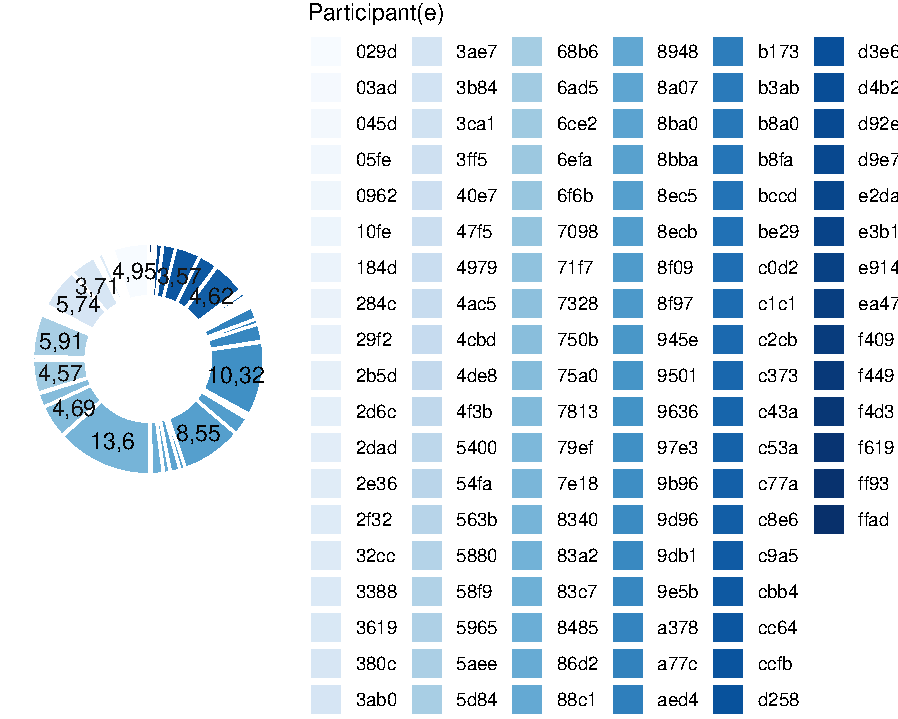
\includegraphics{Images/Pourcent_participant.pdf}}
\end{center}


\subsection{Graphiques relatifs aux mesures}

Pour la répartition des mesures en fonction de la période de la journée :
\begin{knitrout}\footnotesize
\definecolor{shadecolor}{rgb}{0.91, 0.91, 0.91}\color{fgcolor}\begin{kframe}
\begin{alltt}
\hlstd{p} \hlkwb{<-} \hlkwd{ggplot}\hlstd{(data_mes,} \hlkwd{aes}\hlstd{(}\hlkwc{x} \hlstd{=} \hlkwd{factor}\hlstd{(DateHeure)))} \hlopt{+}
  \hlkwd{geom_bar}\hlstd{(}\hlkwc{fill}\hlstd{=}\hlstr{"steelblue4"}\hlstd{)} \hlopt{+}
  \hlkwd{scale_y_continuous}\hlstd{(}\hlkwc{labels}\hlstd{=}\hlkwa{function}\hlstd{(}\hlkwc{x}\hlstd{)} \hlkwd{format}\hlstd{(x,} \hlkwc{big.mark} \hlstd{=} \hlstr{" "}\hlstd{,} \hlkwc{scientific} \hlstd{=} \hlnum{FALSE}\hlstd{),} \hlkwc{name}\hlstd{=}\hlstr{"Effectif"}\hlstd{)} \hlopt{+}
  \hlkwd{scale_x_discrete}\hlstd{(}\hlstr{"Heure"}\hlstd{)}
\hlkwd{ggsave}\hlstd{(}\hlkwc{device}\hlstd{=}\hlstr{"pdf"}\hlstd{,} \hlkwd{here}\hlstd{(}\hlstr{"Images"}\hlstd{,}\hlstr{"Distrib_heure.pdf"}\hlstd{),p)}
\hlkwd{ggsave}\hlstd{(}\hlkwc{device}\hlstd{=}\hlstr{"jpeg"}\hlstd{,} \hlkwd{here}\hlstd{(}\hlstr{"Images"}\hlstd{,}\hlstr{"Distrib_heure.jpeg"}\hlstd{),p)}
\end{alltt}
\end{kframe}
\end{knitrout}

\begin{center}
\scalebox{.5}{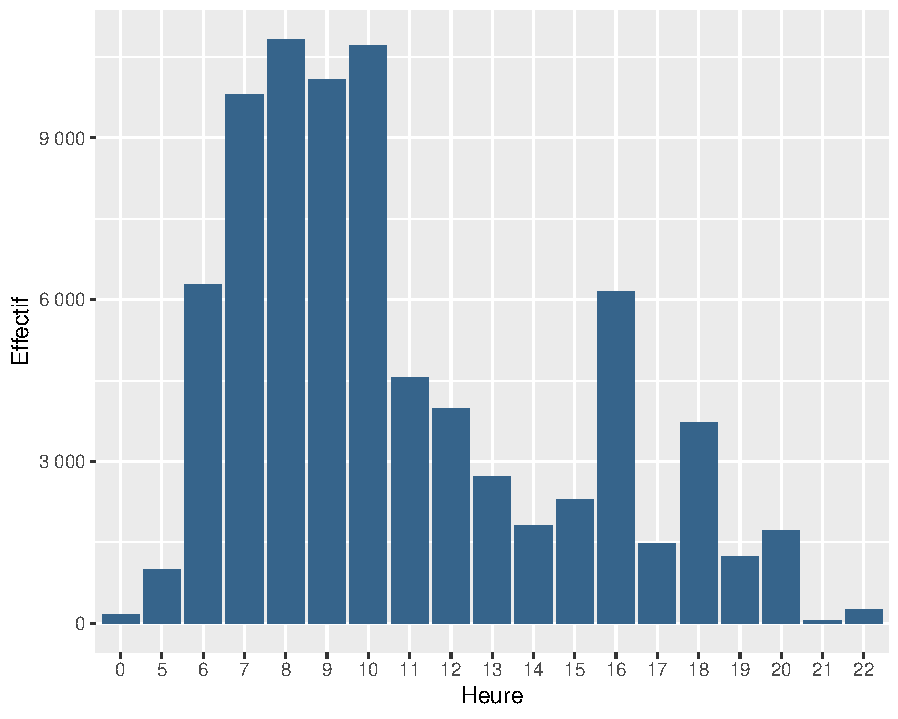
\includegraphics{Images/Distrib_heure.pdf}}
\end{center}

Pour la représentation graphique conjointe des nombre et nombre cumulé de mesures par jour, on a besoin de passer le tableau de données au format long (c.-à-d. de créer une colonne appelée \type{type} et comportant les valeurs \type{NbMes} et \type{NbMesCum}) :
\begin{knitrout}\footnotesize
\definecolor{shadecolor}{rgb}{0.91, 0.91, 0.91}\color{fgcolor}\begin{kframe}
\begin{alltt}
\hlstd{p} \hlkwb{<-}\hlstd{data_mes_jour} \hlopt
  \hlkwd{gather}\hlstd{(.,} \hlkwc{key}\hlstd{=}\hlstr{"type"}\hlstd{,}\hlkwc{value}\hlstd{=}\hlstr{"value"}\hlstd{,NbMes, NbMesCum)} \hlopt \hlcom{#on passe au format long des données}
  \hlkwd{mutate}\hlstd{(}\hlkwc{DateJour}\hlstd{=}\hlkwd{as.Date}\hlstd{(DateJour,} \hlkwc{format} \hlstd{=} \hlstr{"%d.%m.%Y"}\hlstd{))} \hlopt
  \hlkwd{mutate}\hlstd{(}\hlkwc{type} \hlstd{=} \hlkwd{recode}\hlstd{(type,} \hlkwc{NbMes} \hlstd{=} \hlstr{"Journalier"}\hlstd{,} \hlkwc{NbMesCum} \hlstd{=} \hlstr{"Cumulé"}\hlstd{))} \hlopt
  \hlkwd{as.data.frame}\hlstd{()} \hlopt
  \hlkwd{ggplot}\hlstd{(}\hlkwd{aes}\hlstd{(}\hlkwc{x}\hlstd{=DateJour,} \hlkwc{y}\hlstd{=value,} \hlkwc{fill}\hlstd{=type))} \hlopt{+}
  \hlkwd{geom_col}\hlstd{(}\hlkwc{width}\hlstd{=}\hlnum{0.4}\hlstd{,} \hlkwc{position}\hlstd{=}\hlkwd{position_dodge}\hlstd{(}\hlkwc{width}\hlstd{=}\hlnum{0.5}\hlstd{))} \hlopt{+}
  \hlkwd{scale_fill_manual}\hlstd{(}\hlkwc{values}\hlstd{=}\hlkwd{c}\hlstd{(}\hlstr{"#10A8E3"}\hlstd{,}\hlstr{"#0A749F"}\hlstd{),} \hlkwc{name}\hlstd{=}\hlstr{"Nombre de mesures"}\hlstd{)} \hlopt{+}
  \hlkwd{scale_y_continuous}\hlstd{(}\hlkwc{labels}\hlstd{=}\hlkwa{function}\hlstd{(}\hlkwc{x}\hlstd{)} \hlkwd{format}\hlstd{(x,} \hlkwc{big.mark} \hlstd{=} \hlstr{" "}\hlstd{,} \hlkwc{scientific} \hlstd{=} \hlnum{FALSE}\hlstd{),} \hlkwc{name}\hlstd{=}\hlstr{"Effectif"}\hlstd{)} \hlopt{+}
  \hlkwd{scale_x_date}\hlstd{(}\hlkwc{breaks} \hlstd{= data_mes_jour}\hlopt{$}\hlstd{DateJour,} \hlkwc{name}\hlstd{=}\hlstr{"Date"}\hlstd{,} \hlkwc{date_labels} \hlstd{=} \hlstr{"%d/%m"}\hlstd{)} \hlopt{+}
  \hlkwd{theme}\hlstd{(}\hlkwc{axis.text.x} \hlstd{=} \hlkwd{element_text}\hlstd{(}\hlkwc{size}\hlstd{=}\hlnum{8}\hlstd{,} \hlkwc{angle}\hlstd{=}\hlnum{45}\hlstd{))} \hlopt{+}
  \hlkwd{guides}\hlstd{(}\hlkwc{fill} \hlstd{=} \hlkwd{guide_legend}\hlstd{(}\hlkwc{reverse}\hlstd{=}\hlnum{TRUE}\hlstd{))}
\hlkwd{ggsave}\hlstd{(}\hlkwc{device}\hlstd{=}\hlstr{"pdf"}\hlstd{,} \hlkwd{here}\hlstd{(}\hlstr{"Images"}\hlstd{,}\hlstr{"Mesures_distrib_jour.pdf"}\hlstd{),p)}
\hlkwd{ggsave}\hlstd{(}\hlkwc{device}\hlstd{=}\hlstr{"jpeg"}\hlstd{,} \hlkwd{here}\hlstd{(}\hlstr{"Images"}\hlstd{,}\hlstr{"Mesures_distrib_jour.jpeg"}\hlstd{),p)}
\end{alltt}
\end{kframe}
\end{knitrout}

\begin{center}
\scalebox{.5}{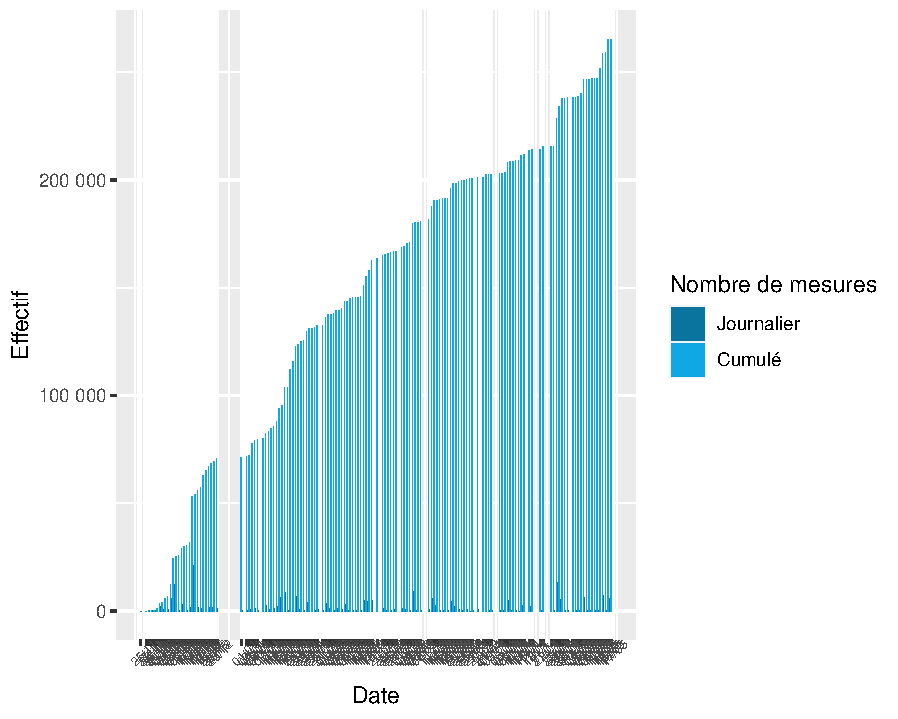
\includegraphics{Images/Mesures_distrib_jour.pdf}}
\end{center}


\subsection{Graphiques relatifs aux traces}

Pour la représentation graphique conjointe des nombre et nombre cumulé de traces par jour, il est encore nécessaire de passer au format long :
\begin{knitrout}\footnotesize
\definecolor{shadecolor}{rgb}{0.91, 0.91, 0.91}\color{fgcolor}\begin{kframe}
\begin{alltt}
\hlstd{p} \hlkwb{<-} \hlstd{data_trace_jour} \hlopt
  \hlkwd{gather}\hlstd{(.,} \hlkwc{key}\hlstd{=}\hlstr{"type"}\hlstd{,}\hlkwc{value}\hlstd{=}\hlstr{"value"}\hlstd{,NbTraceParJour, NbTraceParJourCum)} \hlopt \hlcom{#on passe au format long des données}
  \hlkwd{mutate}\hlstd{(}\hlkwc{DateJour}\hlstd{=}\hlkwd{as.Date}\hlstd{(DateJour,} \hlkwc{format} \hlstd{=} \hlstr{"%d.%m.%Y"}\hlstd{))} \hlopt
  \hlkwd{mutate}\hlstd{(}\hlkwc{type} \hlstd{=} \hlkwd{recode}\hlstd{(type,} \hlkwc{NbTraceParJour} \hlstd{=} \hlstr{"Journalier"}\hlstd{,} \hlkwc{NbTraceParJourCum} \hlstd{=} \hlstr{"Cumulé"}\hlstd{))} \hlopt
  \hlkwd{as.data.frame}\hlstd{()} \hlopt
  \hlkwd{ggplot}\hlstd{(}\hlkwd{aes}\hlstd{(}\hlkwc{x}\hlstd{=DateJour,} \hlkwc{y}\hlstd{=value,} \hlkwc{fill}\hlstd{=type))} \hlopt{+}
  \hlkwd{geom_col}\hlstd{(}\hlkwc{width}\hlstd{=}\hlnum{0.4}\hlstd{,} \hlkwc{position}\hlstd{=}\hlkwd{position_dodge}\hlstd{(}\hlkwc{width}\hlstd{=}\hlnum{0.5}\hlstd{))} \hlopt{+}
  \hlkwd{scale_fill_manual}\hlstd{(}\hlkwc{values}\hlstd{=}\hlkwd{c}\hlstd{(}\hlstr{"#10A8E3"}\hlstd{,}\hlstr{"#0A749F"}\hlstd{),} \hlkwc{name}\hlstd{=}\hlstr{"Nombre de traces"}\hlstd{)} \hlopt{+}
  \hlkwd{scale_y_continuous}\hlstd{(}\hlkwc{name}\hlstd{=}\hlstr{"Effectif"}\hlstd{)} \hlopt{+}
  \hlkwd{scale_x_date}\hlstd{(}\hlkwc{breaks} \hlstd{= data_trace_jour}\hlopt{$}\hlstd{DateJour,} \hlkwc{name}\hlstd{=}\hlstr{"Date"}\hlstd{,} \hlkwc{date_labels} \hlstd{=} \hlstr{"%d/%m"}\hlstd{)} \hlopt{+}
  \hlkwd{theme}\hlstd{(}\hlkwc{axis.text.x} \hlstd{=} \hlkwd{element_text}\hlstd{(}\hlkwc{size}\hlstd{=}\hlnum{8}\hlstd{,} \hlkwc{angle}\hlstd{=}\hlnum{45}\hlstd{))} \hlopt{+}
  \hlkwd{guides}\hlstd{(}\hlkwc{fill} \hlstd{=} \hlkwd{guide_legend}\hlstd{(}\hlkwc{reverse}\hlstd{=}\hlnum{TRUE}\hlstd{))}
\hlkwd{ggsave}\hlstd{(}\hlkwc{device}\hlstd{=}\hlstr{"pdf"}\hlstd{,} \hlkwd{here}\hlstd{(}\hlstr{"Images"}\hlstd{,}\hlstr{"Traces_distrib_jour.pdf"}\hlstd{),p)}
\hlkwd{ggsave}\hlstd{(}\hlkwc{device}\hlstd{=}\hlstr{"jpeg"}\hlstd{,} \hlkwd{here}\hlstd{(}\hlstr{"Images"}\hlstd{,}\hlstr{"Traces_distrib_jour.jpeg"}\hlstd{),p)}
\end{alltt}
\end{kframe}
\end{knitrout}

\begin{center}
\scalebox{.5}{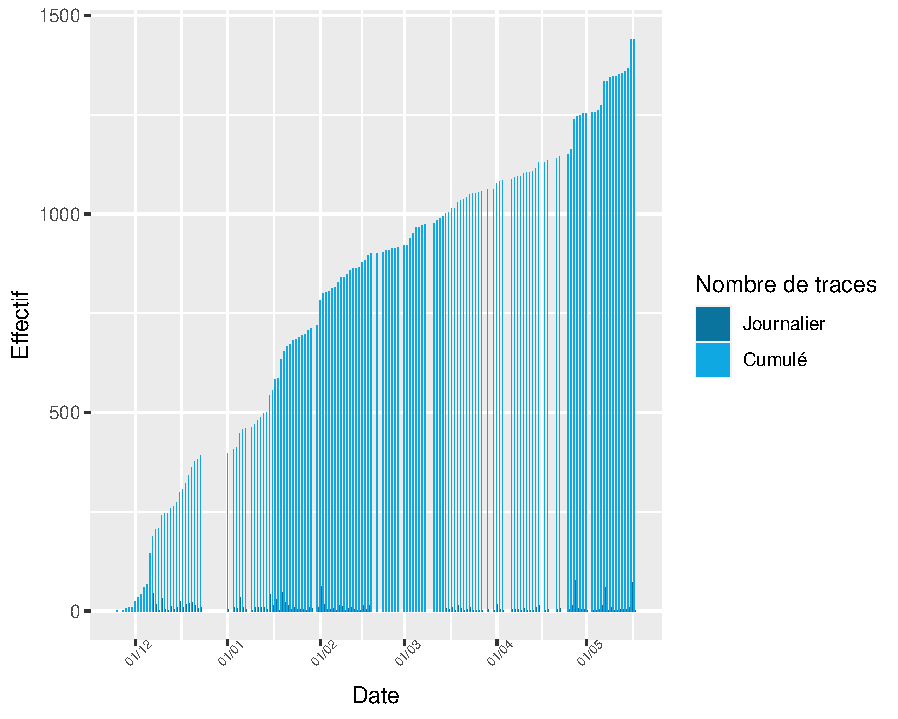
\includegraphics{Images/Traces_distrib_jour.pdf}}
\end{center}

Pour la représentation graphique conjointe des nombre et nombre cumulé de traces par jour de la semaine :
\begin{knitrout}\footnotesize
\definecolor{shadecolor}{rgb}{0.91, 0.91, 0.91}\color{fgcolor}\begin{kframe}
\begin{alltt}
\hlstd{p} \hlkwb{<-} \hlstd{data_trace_jour} \hlopt
  \hlkwd{mutate}\hlstd{(}\hlkwc{JourJ}\hlstd{=}\hlkwd{wday}\hlstd{(}\hlkwd{as.POSIXct}\hlstd{(DateJour),} \hlkwc{label} \hlstd{=} \hlnum{TRUE}\hlstd{,} \hlkwc{abbr}\hlstd{=}\hlnum{FALSE}\hlstd{))} \hlopt
  \hlkwd{mutate}\hlstd{(}\hlkwc{JourJ} \hlstd{=} \hlkwd{factor}\hlstd{(JourJ))} \hlopt
  \hlkwd{mutate}\hlstd{(}\hlkwc{JourJ}\hlstd{=}\hlkwd{fct_relevel}\hlstd{(JourJ,}\hlkwd{c}\hlstd{(}\hlstr{"Lundi"}\hlstd{,}\hlstr{"Mardi"}\hlstd{,}\hlstr{"Mercredi"}\hlstd{,}\hlstr{"Jeudi"}\hlstd{,}\hlstr{"Vendredi"}\hlstd{,}\hlstr{"Samedi"}\hlstd{,}\hlstr{"Dimanche"}\hlstd{)))} \hlopt
  \hlkwd{arrange}\hlstd{(JourJ)} \hlopt
  \hlkwd{as.data.frame}\hlstd{()} \hlopt
  \hlkwd{ggplot}\hlstd{(}\hlkwd{aes}\hlstd{(}\hlkwc{x}\hlstd{=JourJ,}\hlkwc{y}\hlstd{=NbTraceParJour,}\hlkwc{fill}\hlstd{=JourJ))} \hlopt{+}
  \hlkwd{geom_col}\hlstd{(}\hlkwc{width}\hlstd{=}\hlnum{0.4}\hlstd{,} \hlkwc{fill}\hlstd{=}\hlstr{"#0A749F"}\hlstd{)} \hlopt{+}
  \hlkwd{scale_y_continuous}\hlstd{(}\hlkwc{name}\hlstd{=}\hlstr{"Effectif"}\hlstd{)} \hlopt{+}
  \hlkwd{scale_x_discrete}\hlstd{(}\hlkwc{name}\hlstd{=}\hlstr{"Jour de la semaine"}\hlstd{)} \hlopt{+}
  \hlkwd{theme}\hlstd{(}\hlkwc{axis.text.x} \hlstd{=} \hlkwd{element_text}\hlstd{(}\hlkwc{size}\hlstd{=}\hlnum{8}\hlstd{))} \hlopt{+}
  \hlkwd{theme}\hlstd{(}\hlkwc{legend.position} \hlstd{=} \hlstr{"none"}\hlstd{)}
\hlkwd{ggsave}\hlstd{(}\hlkwc{device}\hlstd{=}\hlstr{"pdf"}\hlstd{,} \hlkwd{here}\hlstd{(}\hlstr{"Images"}\hlstd{,}\hlstr{"Traces_distrib_joursem.pdf"}\hlstd{),p)}
\hlkwd{ggsave}\hlstd{(}\hlkwc{device}\hlstd{=}\hlstr{"jpeg"}\hlstd{,} \hlkwd{here}\hlstd{(}\hlstr{"Images"}\hlstd{,}\hlstr{"Traces_distrib_joursem.jpeg"}\hlstd{),p)}
\end{alltt}
\end{kframe}
\end{knitrout}

\begin{center}
\scalebox{.5}{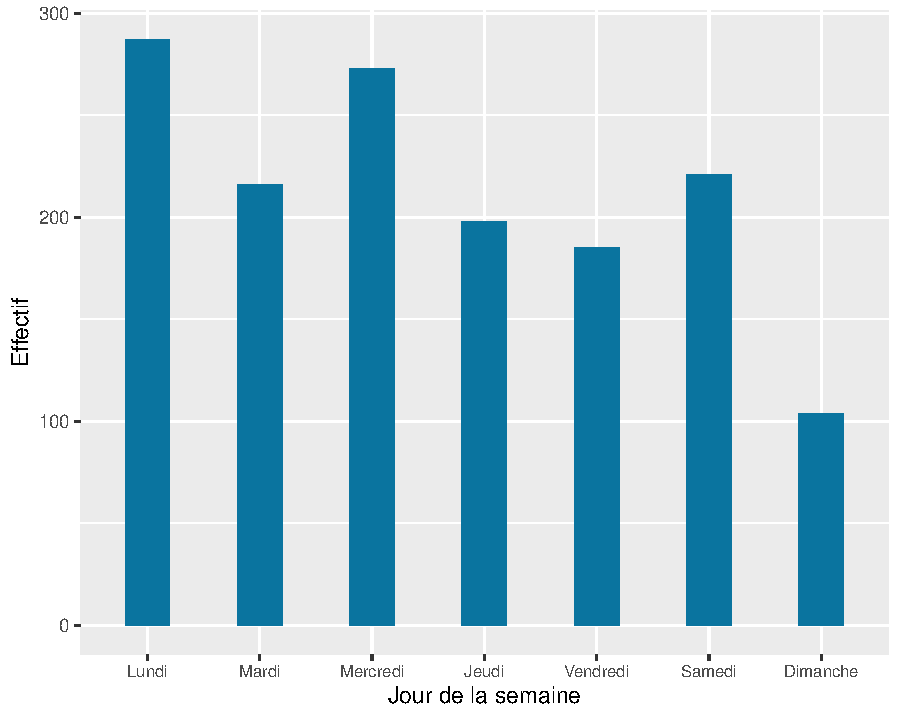
\includegraphics{Images/Traces_distrib_joursem.pdf}}
\end{center}

On va ensuite afficher la répartition des traces par plages de durées. D'emblée, pour avoir une échelle telle que les résultats soient lisibles, on va distinguer les traces dont la durée est inférieure à 5~min des autres.

Pour les traces de courte durée :
\begin{knitrout}\footnotesize
\definecolor{shadecolor}{rgb}{0.91, 0.91, 0.91}\color{fgcolor}\begin{kframe}
\begin{alltt}
\hlstd{trace_classe_inf5} \hlkwb{<-} \hlstd{data_trace} \hlopt
  \hlkwd{filter}\hlstd{(DureeMinutes} \hlopt{<=} \hlnum{5}\hlstd{)} \hlopt
  \hlkwd{mutate}\hlstd{(}\hlkwc{Classe} \hlstd{=} \hlkwd{case_when}\hlstd{(DureeMinutes} \hlopt{<} \hlnum{1} \hlopt{~} \hlstr{"0-1"}\hlstd{,}
                            \hlstd{DureeMinutes} \hlopt{<} \hlnum{2} \hlopt{~} \hlstr{"1-2"}\hlstd{,}
                            \hlstd{DureeMinutes} \hlopt{<} \hlnum{3} \hlopt{~} \hlstr{"2-3"}\hlstd{,}
                            \hlstd{DureeMinutes} \hlopt{<} \hlnum{4} \hlopt{~} \hlstr{"3-4"}\hlstd{,}
                            \hlnum{TRUE} \hlopt{~} \hlstr{"4-5"}\hlstd{))} \hlopt
  \hlkwd{mutate}\hlstd{(}\hlkwc{Classe} \hlstd{=} \hlkwd{factor}\hlstd{(Classe))}
\hlkwd{levels}\hlstd{(trace_classe_inf5}\hlopt{$}\hlstd{Classe)}

\hlstd{trace_classe_inf5} \hlkwb{<-} \hlstd{trace_classe_inf5} \hlopt
  \hlkwd{distinct}\hlstd{(IdTrace,} \hlkwc{.keep_all} \hlstd{=} \hlnum{TRUE}\hlstd{)} \hlopt
  \hlkwd{mutate}\hlstd{(}\hlkwc{Classe} \hlstd{= forcats}\hlopt{::}\hlkwd{fct_relevel}\hlstd{(Classe,}\hlkwd{c}\hlstd{(}\hlstr{"0-1"}\hlstd{,}\hlstr{"1-2"}\hlstd{,}\hlstr{"2-3"}\hlstd{,}\hlstr{"3-4"}\hlstd{,}\hlstr{"4-5"}\hlstd{)))} \hlopt
  \hlkwd{arrange}\hlstd{(Classe)}
\hlkwd{levels}\hlstd{(trace_classe_inf5}\hlopt{$}\hlstd{Classe)}

\hlstd{p} \hlkwb{<-} \hlkwd{ggplot}\hlstd{(trace_classe_inf5,}\hlkwd{aes}\hlstd{(}\hlkwc{x} \hlstd{= Classe))} \hlopt{+}
  \hlkwd{geom_bar}\hlstd{(}\hlkwc{fill}\hlstd{=}\hlstr{"steelblue4"}\hlstd{)} \hlopt{+}
  \hlkwd{scale_x_discrete}\hlstd{(}\hlkwc{name}\hlstd{=}\hlstr{"Plages de durée (en minutes)"}\hlstd{)} \hlopt{+}
  \hlkwd{scale_y_continuous}\hlstd{(}\hlkwc{name}\hlstd{=}\hlstr{"Effectif"}\hlstd{,} \hlkwc{breaks}\hlstd{= scales}\hlopt{::}\hlkwd{pretty_breaks}\hlstd{())}
\hlkwd{ggsave}\hlstd{(}\hlkwc{device}\hlstd{=}\hlstr{"pdf"}\hlstd{,} \hlkwd{here}\hlstd{(}\hlstr{"Images"}\hlstd{,}\hlstr{"Traces_distrib_dureemin.pdf"}\hlstd{),p)}
\hlkwd{ggsave}\hlstd{(}\hlkwc{device}\hlstd{=}\hlstr{"jpeg"}\hlstd{,} \hlkwd{here}\hlstd{(}\hlstr{"Images"}\hlstd{,}\hlstr{"Traces_distrib_dureemin.jpeg"}\hlstd{),p)}
\end{alltt}
\end{kframe}
\end{knitrout}

\begin{center}
\scalebox{.5}{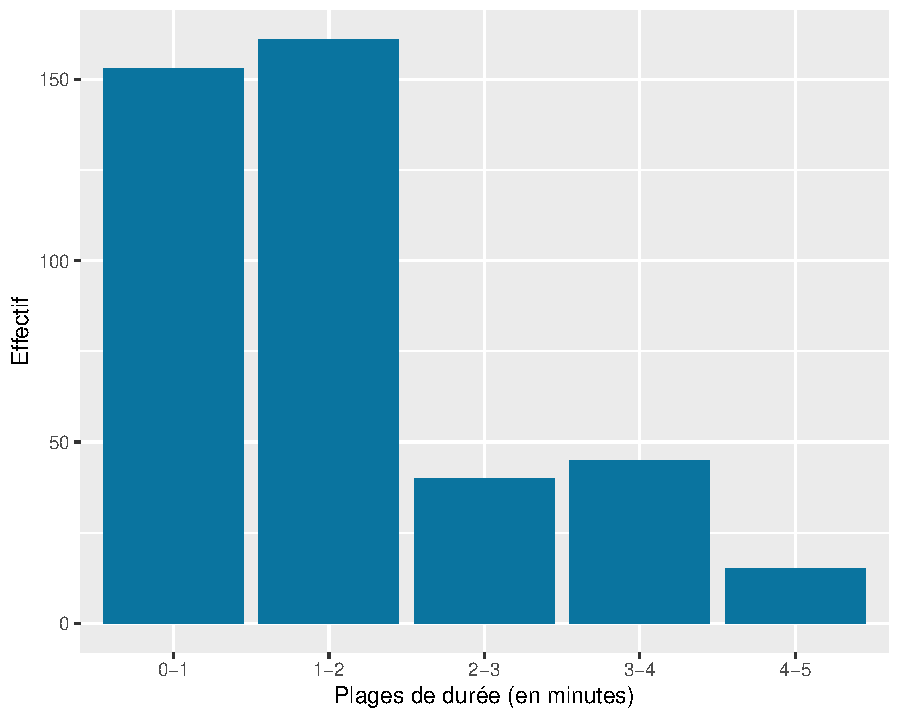
\includegraphics{Images/Traces_distrib_dureemin.pdf}}
\end{center}

Pour les traces de plus longue durée :
\begin{knitrout}\footnotesize
\definecolor{shadecolor}{rgb}{0.91, 0.91, 0.91}\color{fgcolor}\begin{kframe}
\begin{alltt}
\hlstd{trace_classe_sup5} \hlkwb{<-} \hlstd{trace_classe} \hlopt
  \hlkwd{distinct}\hlstd{(IdTrace,} \hlkwc{.keep_all} \hlstd{=} \hlnum{TRUE}\hlstd{)} \hlopt
  \hlkwd{filter}\hlstd{(Classe} \hlopt{!=} \hlstr{"0-5"}\hlstd{)}

\hlkwd{ggplot}\hlstd{(trace_classe_sup5,}\hlkwd{aes}\hlstd{(}\hlkwc{x} \hlstd{= Classe))} \hlopt{+}
  \hlkwd{geom_bar}\hlstd{(}\hlkwc{fill}\hlstd{=}\hlstr{"steelblue4"}\hlstd{)} \hlopt{+}
  \hlkwd{scale_x_discrete}\hlstd{(}\hlkwc{name}\hlstd{=}\hlstr{"Plages de durée (en minutes)"}\hlstd{)} \hlopt{+}
  \hlkwd{scale_y_continuous}\hlstd{(}\hlkwc{name}\hlstd{=}\hlstr{"Effectif"}\hlstd{,} \hlkwc{breaks}\hlstd{= scales}\hlopt{::}\hlkwd{pretty_breaks}\hlstd{())}
\hlkwd{ggsave}\hlstd{(}\hlkwc{device}\hlstd{=}\hlstr{"pdf"}\hlstd{,} \hlkwd{here}\hlstd{(}\hlstr{"Images"}\hlstd{,}\hlstr{"Traces_distrib_dureemax.pdf"}\hlstd{),p)}
\hlkwd{ggsave}\hlstd{(}\hlkwc{device}\hlstd{=}\hlstr{"jpeg"}\hlstd{,} \hlkwd{here}\hlstd{(}\hlstr{"Images"}\hlstd{,}\hlstr{"Traces_distrib_dureemax.jpeg"}\hlstd{),p)}
\end{alltt}
\end{kframe}
\end{knitrout}

\begin{center}
\scalebox{.5}{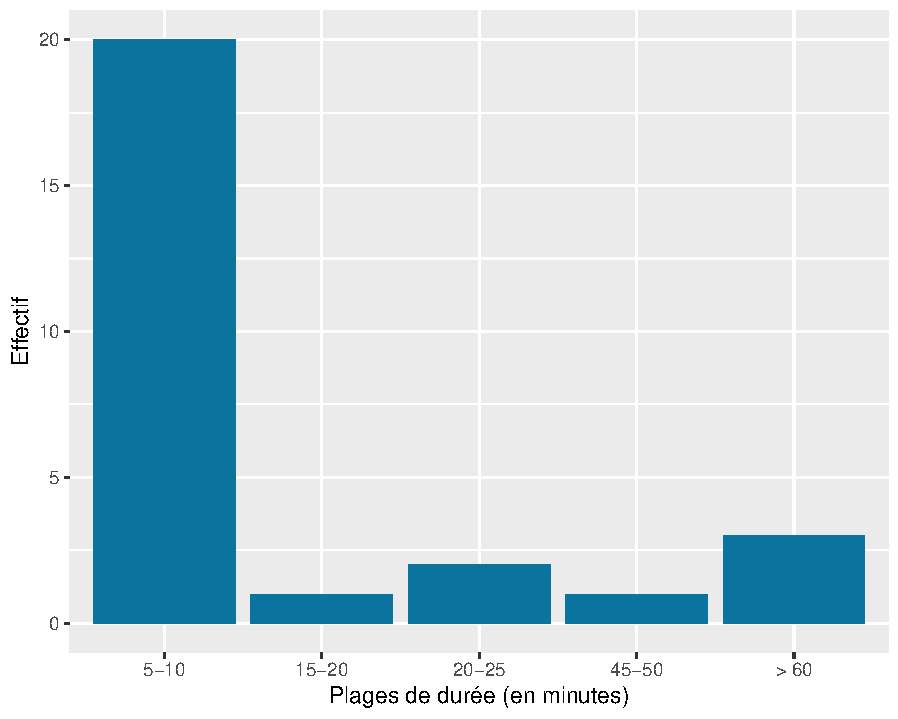
\includegraphics{Images/Traces_distrib_dureemax.pdf}}
\end{center}


\subsection{Carto-graphiques}

Merci à Pierre pour son initiation et le code ci-après ;-)\\[1ex]

À noter qu'en théorie il est possible de sauvegarder directement les cartes dans des fichiers \type{png} grâce au package \type{\{mapview\}} (mais cela ne fonctionne pour l'instant pas pour moi)  :
\begin{knitrout}\footnotesize
\definecolor{shadecolor}{rgb}{0.91, 0.91, 0.91}\color{fgcolor}\begin{kframe}
\begin{alltt}
\hlstd{map} \hlkwb{<-} \hlkwd{leaflet}\hlstd{(...)}
\hlkwd{mapshot}\hlstd{(map,} \hlkwd{here}\hlstd{(}\hlstr{"Images"}\hlstd{,}\hlstr{"Mesures_Polygones.png"}\hlstd{),}\hlkwc{remove_controls} \hlstd{=} \hlkwd{c}\hlstd{(}\hlstr{"zoomControl"}\hlstd{))}
\end{alltt}
\end{kframe}
\end{knitrout}

Il me reste un problème : la mise en page de la légende.

Pour évider un problème d'erreur survenant dans le calcul de la médiane ci-après, et qui exige des variables numériques, on ne retient que les variables d'intérêt :
\begin{knitrout}\footnotesize
\definecolor{shadecolor}{rgb}{0.91, 0.91, 0.91}\color{fgcolor}\begin{kframe}
\begin{alltt}
\hlstd{Data_numerique} \hlkwb{<-} \hlstd{data_nc[,}\hlkwd{c}\hlstd{(}\hlstr{"x"}\hlstd{,}\hlstr{"y"}\hlstd{,}\hlstr{"leq_mean"}\hlstd{)]}
\end{alltt}
\end{kframe}
\end{knitrout}

Ensuite on représente les niveaux de bruits avec des polygones :
\begin{knitrout}\footnotesize
\definecolor{shadecolor}{rgb}{0.91, 0.91, 0.91}\color{fgcolor}\begin{kframe}
\begin{alltt}
\hlstd{SPDF} \hlkwb{<-} \hlkwd{SpatialPointsDataFrame}\hlstd{(}\hlkwc{coords}\hlstd{=Data_numerique[,}\hlnum{1}\hlopt{:}\hlnum{2}\hlstd{],} \hlkwc{data}\hlstd{=}\hlkwd{as.data.frame}\hlstd{(Data_numerique))}
\hlstd{SPDF_sf} \hlkwb{<-} \hlkwd{st_as_sf}\hlstd{(SPDF,} \hlkwc{crs} \hlstd{=} \hlnum{4326}\hlstd{,} \hlkwc{agr} \hlstd{=} \hlstr{"constant"}\hlstd{,} \hlkwc{remove} \hlstd{= F)}
\hlkwd{st_crs}\hlstd{(SPDF_sf)} \hlkwb{<-} \hlnum{4326} \hlcom{#EPSG WGS84}

\hlstd{SPDF_sf_2154} \hlkwb{<-} \hlkwd{st_transform}\hlstd{(SPDF_sf,} \hlnum{2154}\hlstd{)} \hlcom{#LAMBERT 93}

\hlstd{bbox} \hlkwb{<-} \hlkwd{st_bbox}\hlstd{(SPDF_sf_2154)}
\hlstd{grid} \hlkwb{<-} \hlstd{sf}\hlopt{::}\hlkwd{st_make_grid}\hlstd{(}\hlkwd{st_as_sfc}\hlstd{(bbox),}\hlkwc{cellsize} \hlstd{=} \hlnum{50}\hlstd{,} \hlkwc{square} \hlstd{=} \hlnum{FALSE}\hlstd{)}  \hlcom{#Grid of 50 meters}
\hlkwd{st_crs}\hlstd{(grid)} \hlkwb{<-} \hlnum{2154}

\hlstd{stations} \hlkwb{<-} \hlkwd{aggregate}\hlstd{(}\hlkwc{x} \hlstd{= SPDF_sf_2154,} \hlkwc{by} \hlstd{= grid,} \hlkwc{FUN} \hlstd{= median)}         \hlcom{#Calculate median}

\hlstd{stations} \hlkwb{<-} \hlstd{stations} \hlopt
  \hlkwd{drop_na}\hlstd{(geometry)} \hlopt
  \hlkwd{drop_na}\hlstd{(leq_mean)}

\hlstd{stations_sf} \hlkwb{<-} \hlkwd{st_as_sf}\hlstd{(stations,} \hlkwc{crs} \hlstd{=} \hlnum{2154}\hlstd{,} \hlkwc{agr} \hlstd{=} \hlstr{"constant"}\hlstd{,}
                        \hlkwc{remove} \hlstd{= F)}

\hlstd{stations_sf_4326} \hlkwb{<-} \hlstd{stations_sf} \hlopt
  \hlkwd{st_transform}\hlstd{(}\hlnum{4326}\hlstd{)} \hlcom{# repasse en WGS84 (LATti LONgi )}

\hlstd{pal2} \hlkwb{<-} \hlkwd{colorNumeric}\hlstd{(}
  \hlkwc{palette} \hlstd{=} \hlstr{"Blues"}\hlstd{,} \hlcom{#"RdYlGn",}
  \hlcom{#n = 9,}
  \hlkwc{domain} \hlstd{= stations}\hlopt{$}\hlstd{leq_mean,}
  \hlcom{#na.color = "transparent",}
  \hlcom{#reverse = TRUE}
  \hlstd{)}

\hlstd{map} \hlkwb{<-} \hlkwd{leaflet}\hlstd{(stations_sf_4326)} \hlopt
  \hlkwd{addProviderTiles}\hlstd{(providers}\hlopt{$}\hlstd{CartoDB.Positron)} \hlopt
  \hlkwd{addScaleBar}\hlstd{(} \hlkwc{position} \hlstd{=} \hlkwd{c}\hlstd{(}\hlstr{"bottomright"}\hlstd{))}\hlopt
  \hlkwd{addPolygons}\hlstd{(}\hlkwc{color} \hlstd{=} \hlopt{~}\hlkwd{pal2}\hlstd{(leq_mean),} \hlkwc{weight} \hlstd{=} \hlnum{0}\hlstd{,} \hlkwc{smoothFactor} \hlstd{=} \hlnum{0.}\hlstd{,}
              \hlkwc{opacity} \hlstd{=} \hlnum{0.0}\hlstd{,} \hlkwc{fillOpacity} \hlstd{=} \hlnum{0.7}\hlstd{,}
              \hlstd{)} \hlopt
  \hlkwd{addLegend}\hlstd{(}\hlstr{"bottomleft"}\hlstd{,}
            \hlkwc{pal} \hlstd{= pal2,}
            \hlcom{#colors = ~pal2,}
            \hlkwc{values} \hlstd{= stations}\hlopt{$}\hlstd{leq_mean,}
            \hlkwc{title} \hlstd{=} \hlstr{"Niveau moyen de bruit"}\hlstd{,}
            \hlcom{#labels = pal2,}
            \hlkwc{labFormat} \hlstd{=} \hlkwd{labelFormat}\hlstd{(}\hlkwc{suffix} \hlstd{=} \hlstr{" dB"}\hlstd{,}\hlkwc{big.mark} \hlstd{=} \hlstr{" "}\hlstd{,} \hlkwc{transform} \hlstd{= identity),}
            \hlkwc{opacity} \hlstd{=} \hlnum{1}
            \hlstd{)}
\hlstd{map}
\hlcom{#}
\hlkwd{mapshot}\hlstd{(map,} \hlkwd{here}\hlstd{(}\hlstr{"Images"}\hlstd{,}\hlstr{"Mesures_Polygones.png"}\hlstd{),}\hlkwc{remove_controls} \hlstd{=} \hlkwd{c}\hlstd{(}\hlstr{"zoomControl"}\hlstd{))}
\end{alltt}
\end{kframe}
\end{knitrout}



\begin{center}
\scalebox{.3}{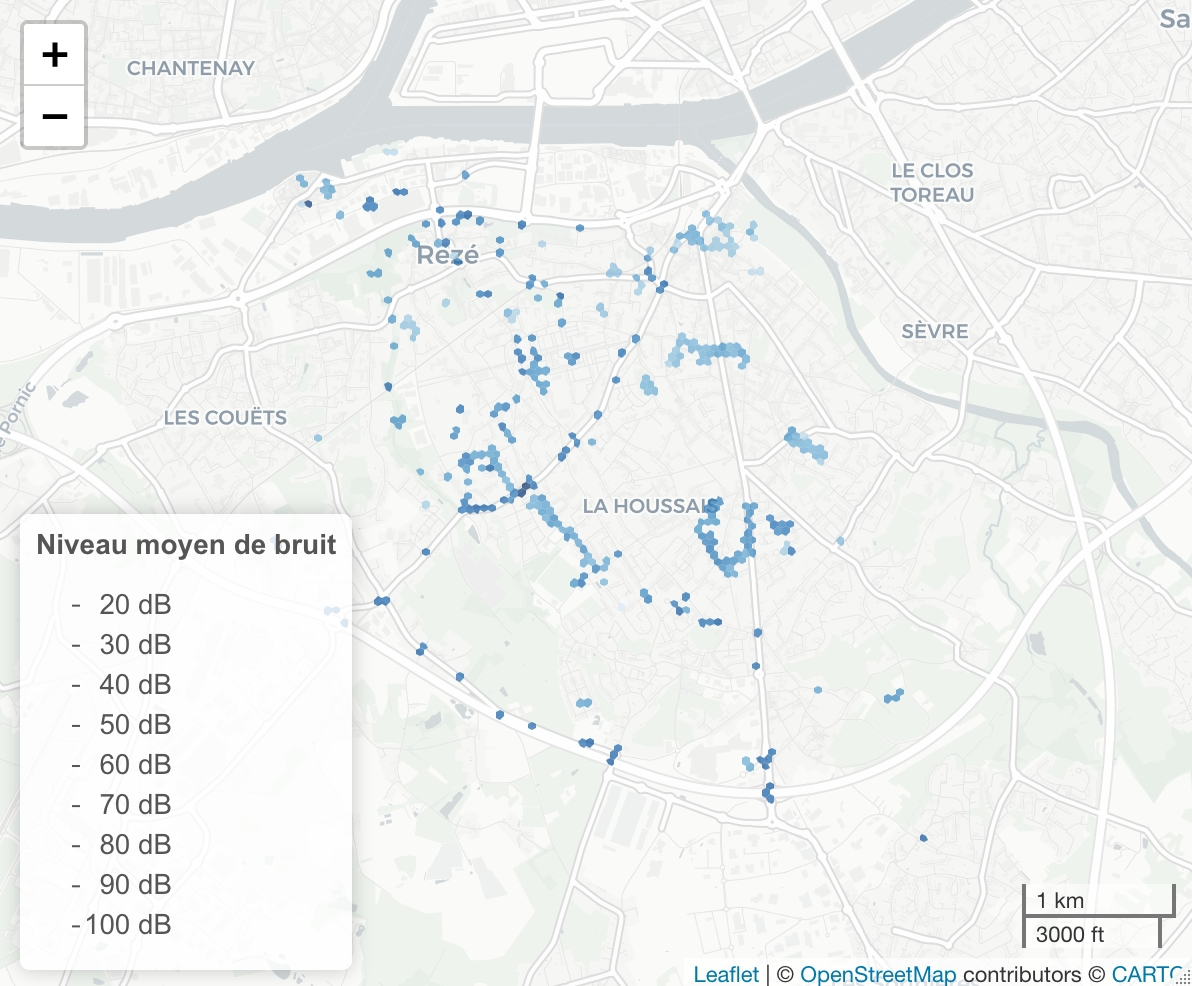
\includegraphics{Images/Carto_polygons.jpeg}}
\end{center}

\end{document}
